%%% -*- coding: utf-8 -*-
\newpage

\chapter{Introdução}
\label{chap:introduction}

Esse é um texto de exemplo para demonstrar algumas funcionalidades do modelo \LaTeX de teses e dissertações da PUC-Rio. As citações são formatadas da seguinte maneira:~\cite{Lee2010},~\cite{Hummel2013},~\cite{Dupacova2003}. 

A idéia desse modelo é a seguinte:

\begin{itemize}
\item Prover um modelo \LaTeX mais atualizado e incorporando algumas correções feitas desde a última versão disponível, lançada em 2017;
\item Prover uma forma mais ágil disponibilizar correções e melhorias do modelo.
\end{itemize}

A Tabela~\ref{tab:cmg-results} apresenta o formato padrão de tabelas desse modelo. Título acima do conteúdo, basicamente. A Figura~\ref{fig:explicit-endoding-szafir} mostra como incluir figuras com subfiguras~(\ref{fig:explicit-encoding-tllamp-inc}, \ref{fig:explicit-endoding-szafir})

\section{Estrutura da Tese}
\label{sec:organization}

\subsection{Subseção de exemplo}

\begin{table}[H]
  \centering
  \caption[Erros dos cenários selecionados usando a abordagem da indústria.]{Cenários escolhidos e erros ($\times 10^{10}$) para a abordagem da indústria.}
  \begin{tabular}{llrrr}
    \hline
    \textbf{Propriedade}       & \textbf{Percentil}       & \textbf{Cenário} & \textbf{SSE}      & \textbf{MSE}   \\ \hline
    \multirow{12}{*}{$N_p$} & \multirow{4}{*}{P$_{10}$} & 172               & 1190.0          & 30.5           \\
                            &                           & 88                & 663.0          & 17.0           \\
                            &                           & 122               & 1660.0          & 42.6           \\
                            &                           & \textbf{36}       & \textbf{312.0} & \textbf{7.9}   \\ \cline{2-5} 
                            & \multirow{4}{*}{P$_{50}$} & 131               & 162.0          & 4.1            \\
                            &                           & \textbf{4}        & \textbf{162.0} & \textbf{4.1}   \\
                            &                           & 26                & 786.0          & 20.1           \\
                            &                           & 90                & 236.0          & 6.0            \\ \cline{2-5} 
                            & \multirow{4}{*}{P$_{90}$} & 96                & 975.0          & 25.0           \\
                            &                           & 100               & 690.0          & 17.7           \\
                            &                           & 127               & 925.0          & 23.7           \\
                            &                           & \textbf{132}      & \textbf{526.0} & \textbf{13.5}  \\ \hline
    \multirow{12}{*}{$W_p$} & \multirow{4}{*}{P$_{10}$} & \textbf{23}       & \textbf{7640.0} & \textbf{196.0} \\
                            &                           & 115               & 42000.0          & 1080.0         \\
                            &                           & 10                & 26900.0          & 690.0          \\
                            &                           & 19                & 27600.0          & 707.0          \\ \cline{2-5} 
                            & \multirow{4}{*}{P$_{50}$} & 29                & 14200.0          & 364.0          \\
                            &                           & 153               & 6260.0          & 161.0          \\
                            &                           & \textbf{84}       & \textbf{5840.0} & \textbf{150.0} \\
                            &                           & 88                & 11200.0          & 288.0          \\ \cline{2-5} 
                            & \multirow{4}{*}{P$_{90}$} & 37                & 14300.0          & 367.0          \\
                            &                           & 57                & 22300.0          & 571.0          \\
                            &                           & 187               & 14000.0          & 358.0          \\
                            &                           & \textbf{28}       & \textbf{2210.0} & \textbf{56.7}  \\ \hline
  \end{tabular}
  \label{tab:cmg-results}
\end{table}

\begin{figure}[H]
  \centering
  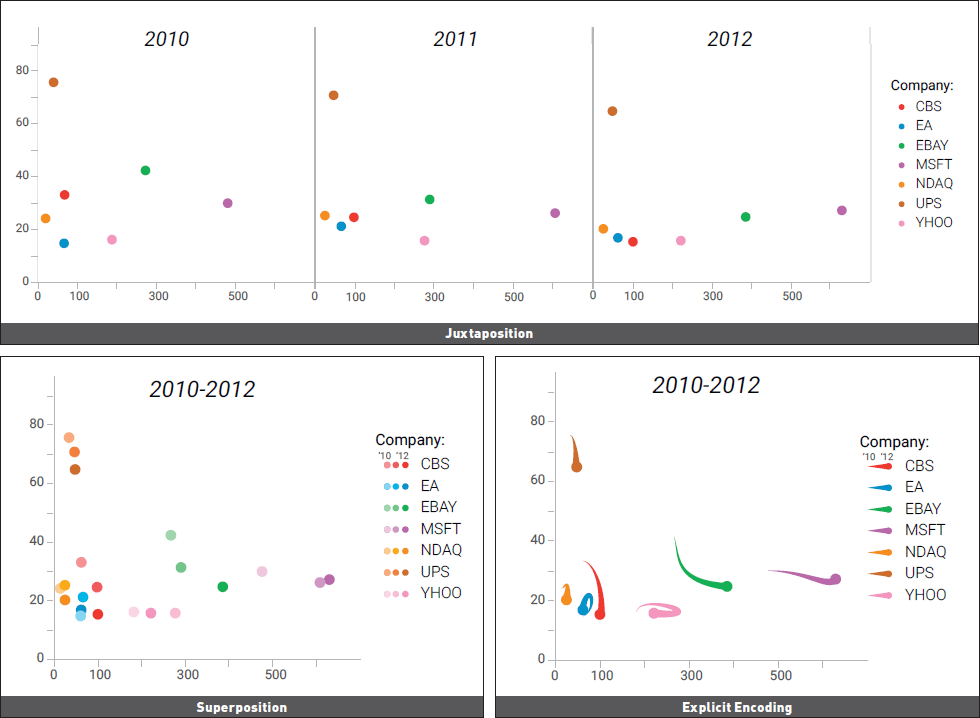
\includegraphics[width=\textwidth]{explicit_encoding}
  \caption{Justaposição, Superposição and Codificação Explícita. Imagem retirada do trabalho de~\cite{Szafir2018}.}
  \label{fig:explicit-endoding-szafir}
\end{figure}

\begin{figure}[H]
  \centering
  \begin{subfigure}[t]{0.75\textwidth}
    \centering
    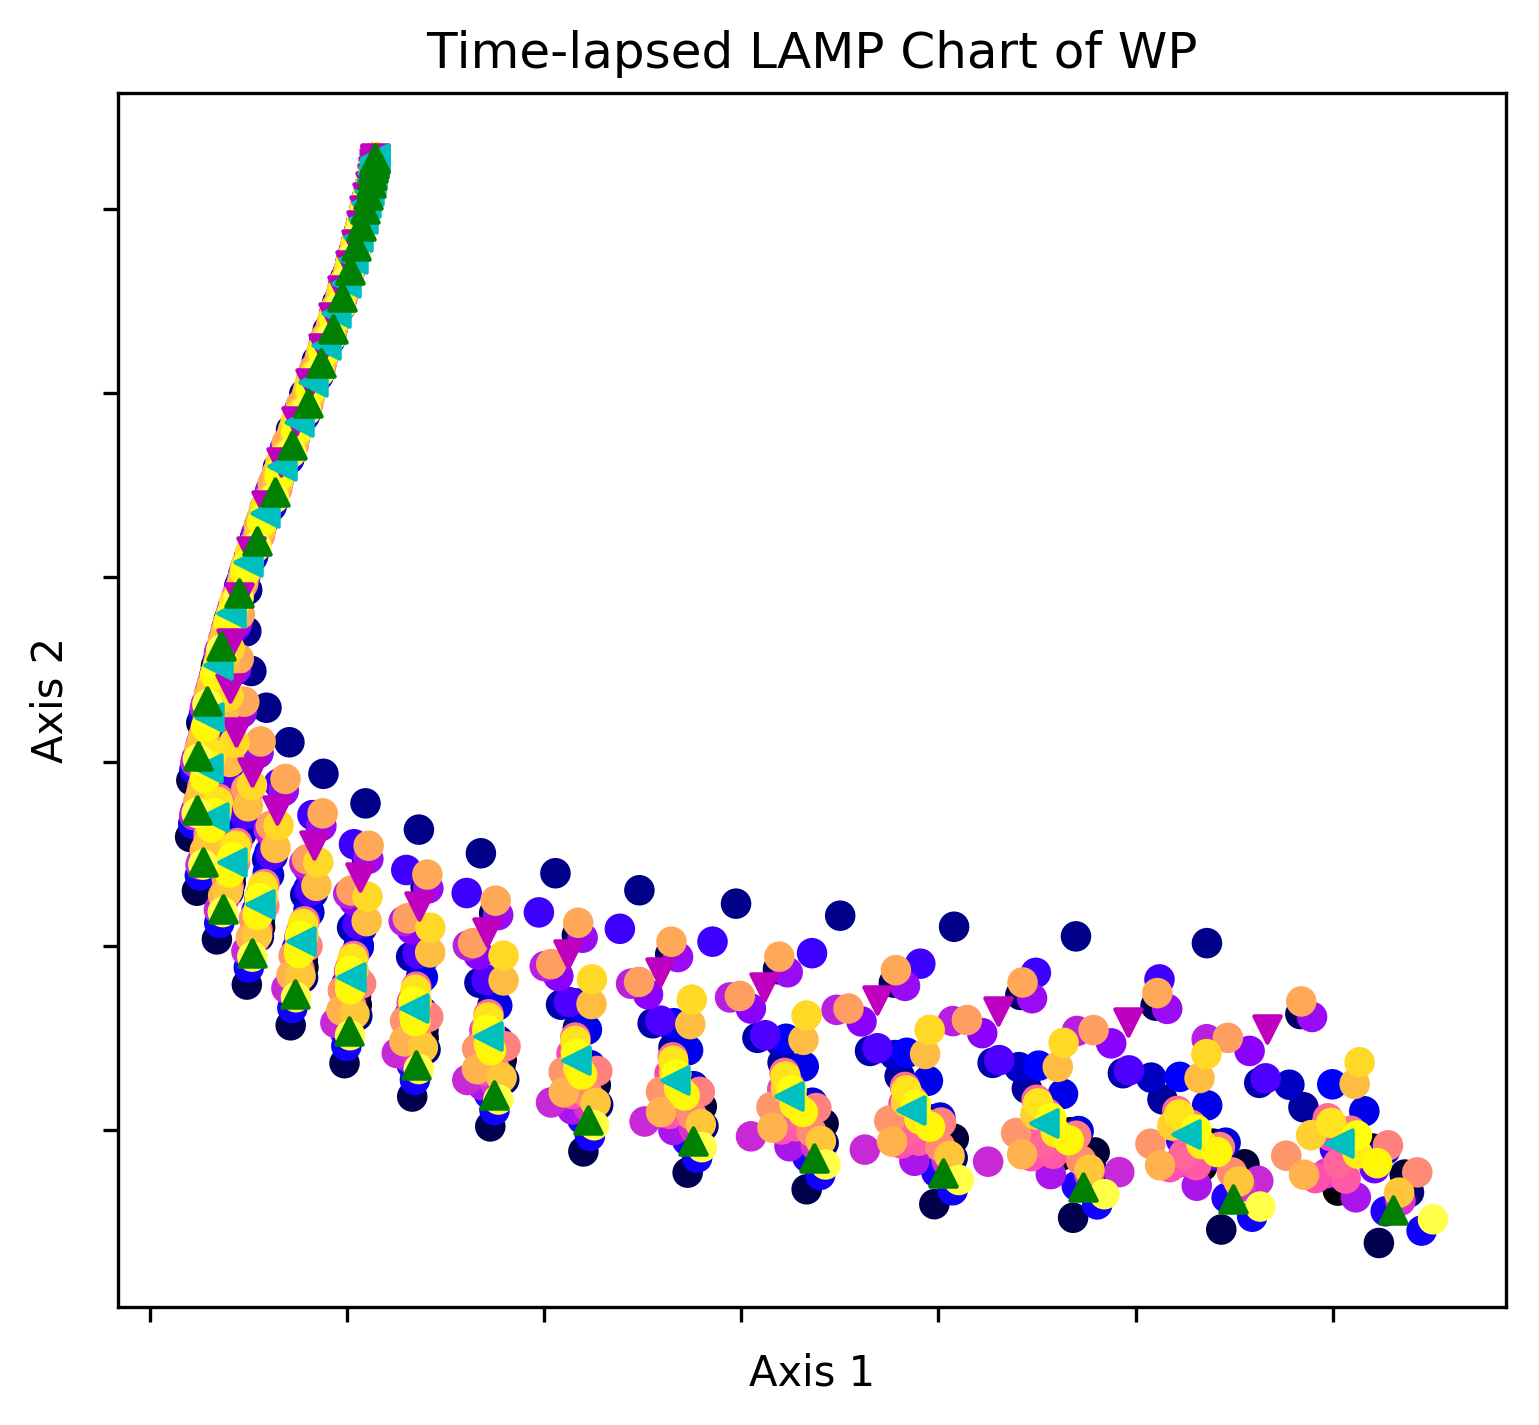
\includegraphics[width=\columnwidth]{WP-tllamp}
    \caption{Superposição de tempos no gráfico Time-lapsed LAMP.}
    \label{fig:superposition-tllamp-inc}
  \end{subfigure}
  ~
  \begin{subfigure}[t]{0.75\textwidth}
    \centering
    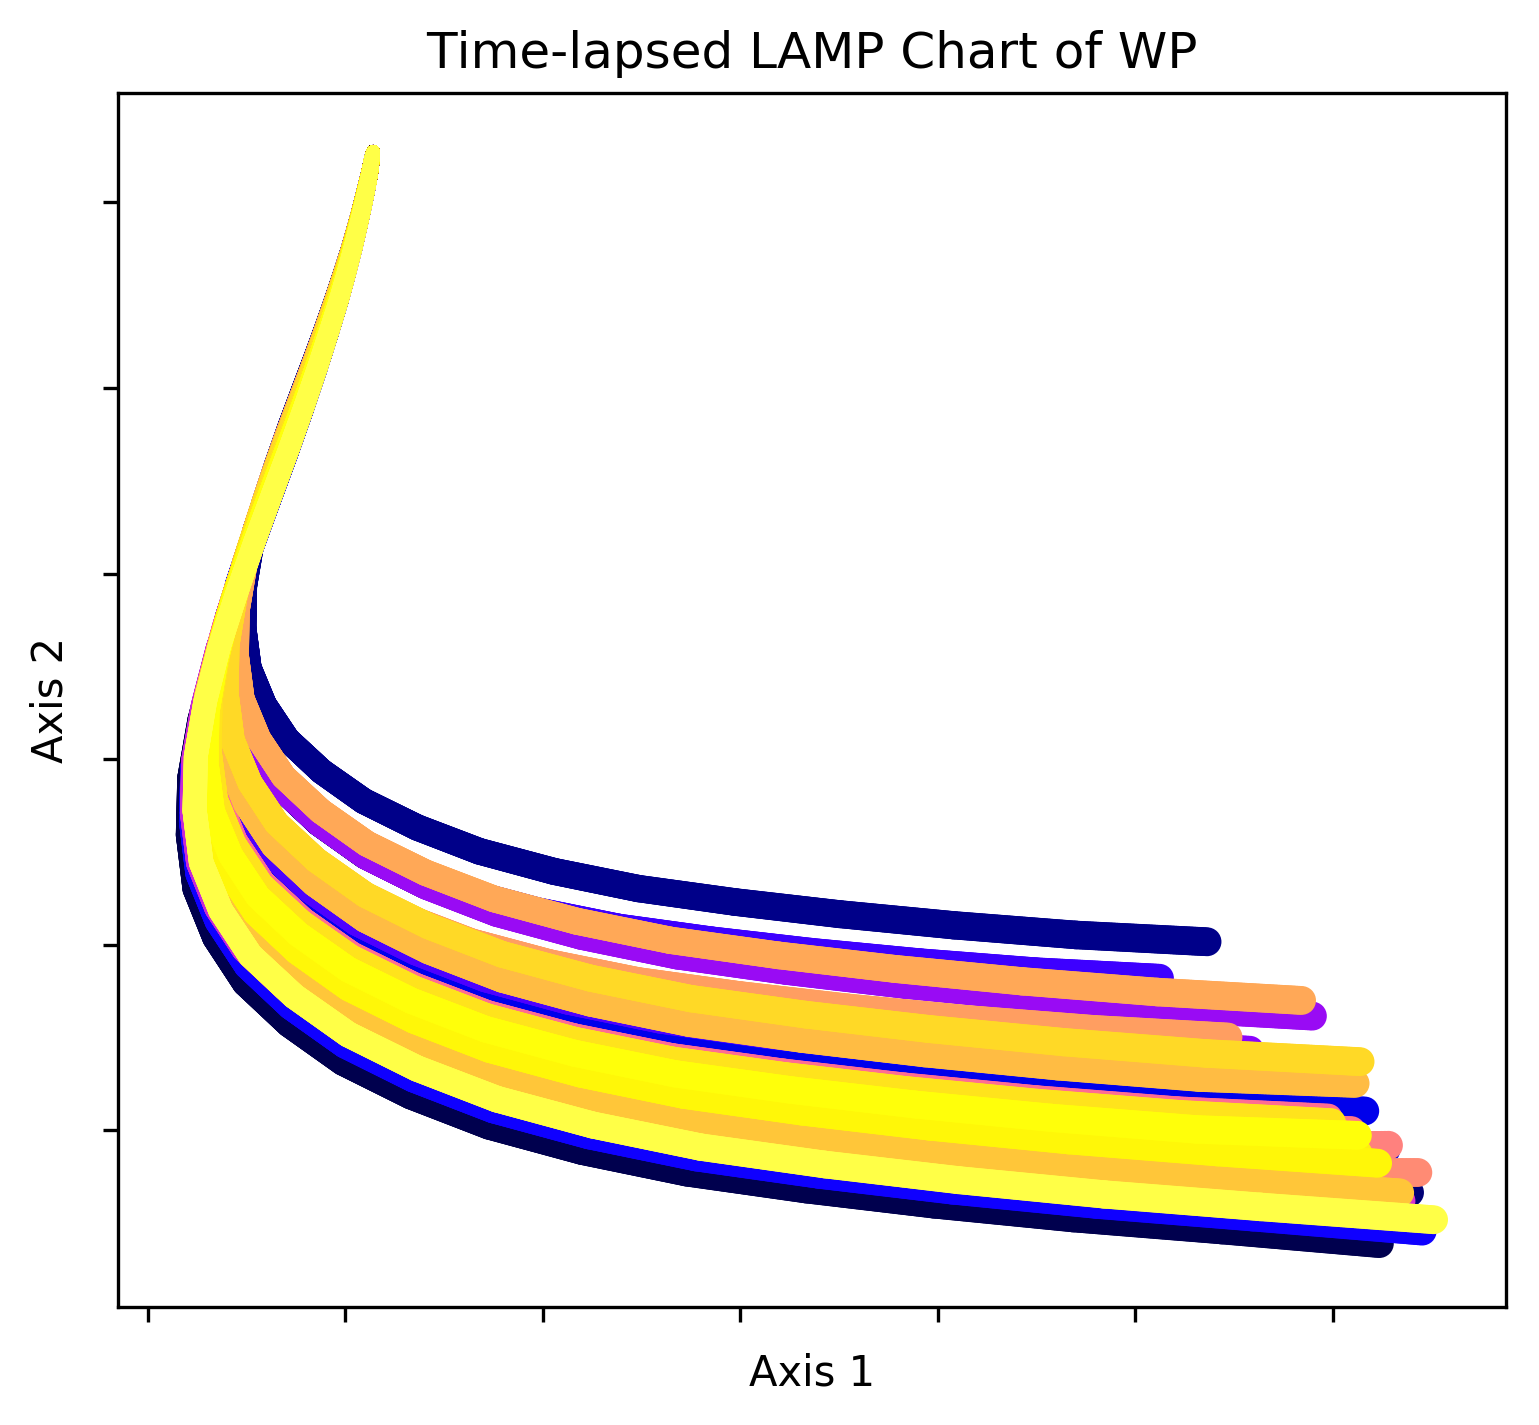
\includegraphics[width=\columnwidth]{WP-tllamp-linear-inc-glyph}
    \caption{Codificação Explícita do tempo no gráfico Time-lapsed LAMP. Tempos iniciais são representados por glifos menores.}
    \label{fig:ee-tllamp-inc}
  \end{subfigure}
  \caption{Comparação entre diferentes representações do tempo para o gráfico Time-lapsed LAMP da propriedade $W_p$. Superposição~(\ref{fig:superposition-tllamp-inc}) e Codificação Explícita~(\ref{fig:ee-tllamp-inc}) em ordem crescente de tamanho de glifo.}
  \label{fig:explicit-encoding-tllamp-inc}
\end{figure}

\subsection{Exemplos de teoremas, lemas e provas}

\begin{theorem}
Dada a função $f$, cuja derivada existe em todos os pontos de seu domínio, então $f$ é chamada função contínua.
\end{theorem}

\begin{theorem}[Teorema de Pitágoras]
\label{pythagorean}
Esse é um teorema que trata de triângulos retângulos, e pode ser sumarizado pela equação a seguir:
\[ x^2 + y^2 = z^2 \]
\end{theorem}

Uma consequência do Teorema~\ref{pythagorean} é o Corolário~\ref{corollary}

\begin{corollary}
\label{corollary}
Não existe triângulo retângulo de lados 3cm, 4cm e 6cm.
\end{corollary}

\begin{lemma}[Operações matriciais que preservam unimodularidade]
  As operações matriciais a seguir, chamadas de operações unimodulares, preservam a unimodularidade de uma matriz se esta for unimodular:
\begin{enumerate}
    \item Troca de duas colunas
    \item Adição de um múltiplo inteiro de uma coluna a outra coluna
    \item Multiplicação de uma coluna por $-1$
    \item Transposição
\end{enumerate}
\end{lemma}

\begin{lemma}
\label{line-segs}
Dados dois segmentos de linha de comprimentos $a$ e $b$ respectivamente, existe um número $r \in \mathbb{R}$ tal que $b=ra$.
\end{lemma}

\begin{proof}
A prova do Lemma~\ref{line-segs} pode ser construída por contradição. Basta assumir que a premissa é falsa e seguir a prova, em algum momento a prova cairá em contradição, portanto, o lema original é verdadeiro.
\end{proof}

%%% Local Variables:
%%% mode: latex
%%% TeX-master: thesis.tex
%%% End:
